\subsubsection{Seriel kommunikation}

SPI forbindelsen blev mellem de to enheder etableret med 6 ledninger som set på figur \ref{ffm_DK8k_PSoC}. En til MOSI, MISO, CLK, SS, VCC og GND.
Udgangen for DevKit8000 er valgt på baggrund af wiki'en for denne enhed\footnote{Se \url{https://redmine.ase.au.dk/devs/projects/devkit8000/wiki/PSOCInterface}}. GPIO-pins på PSoC er valgfrie, og konfigureres 
i PSoC-creator til de ønskede værdier.

\begin{figure}[H]
	\centerline{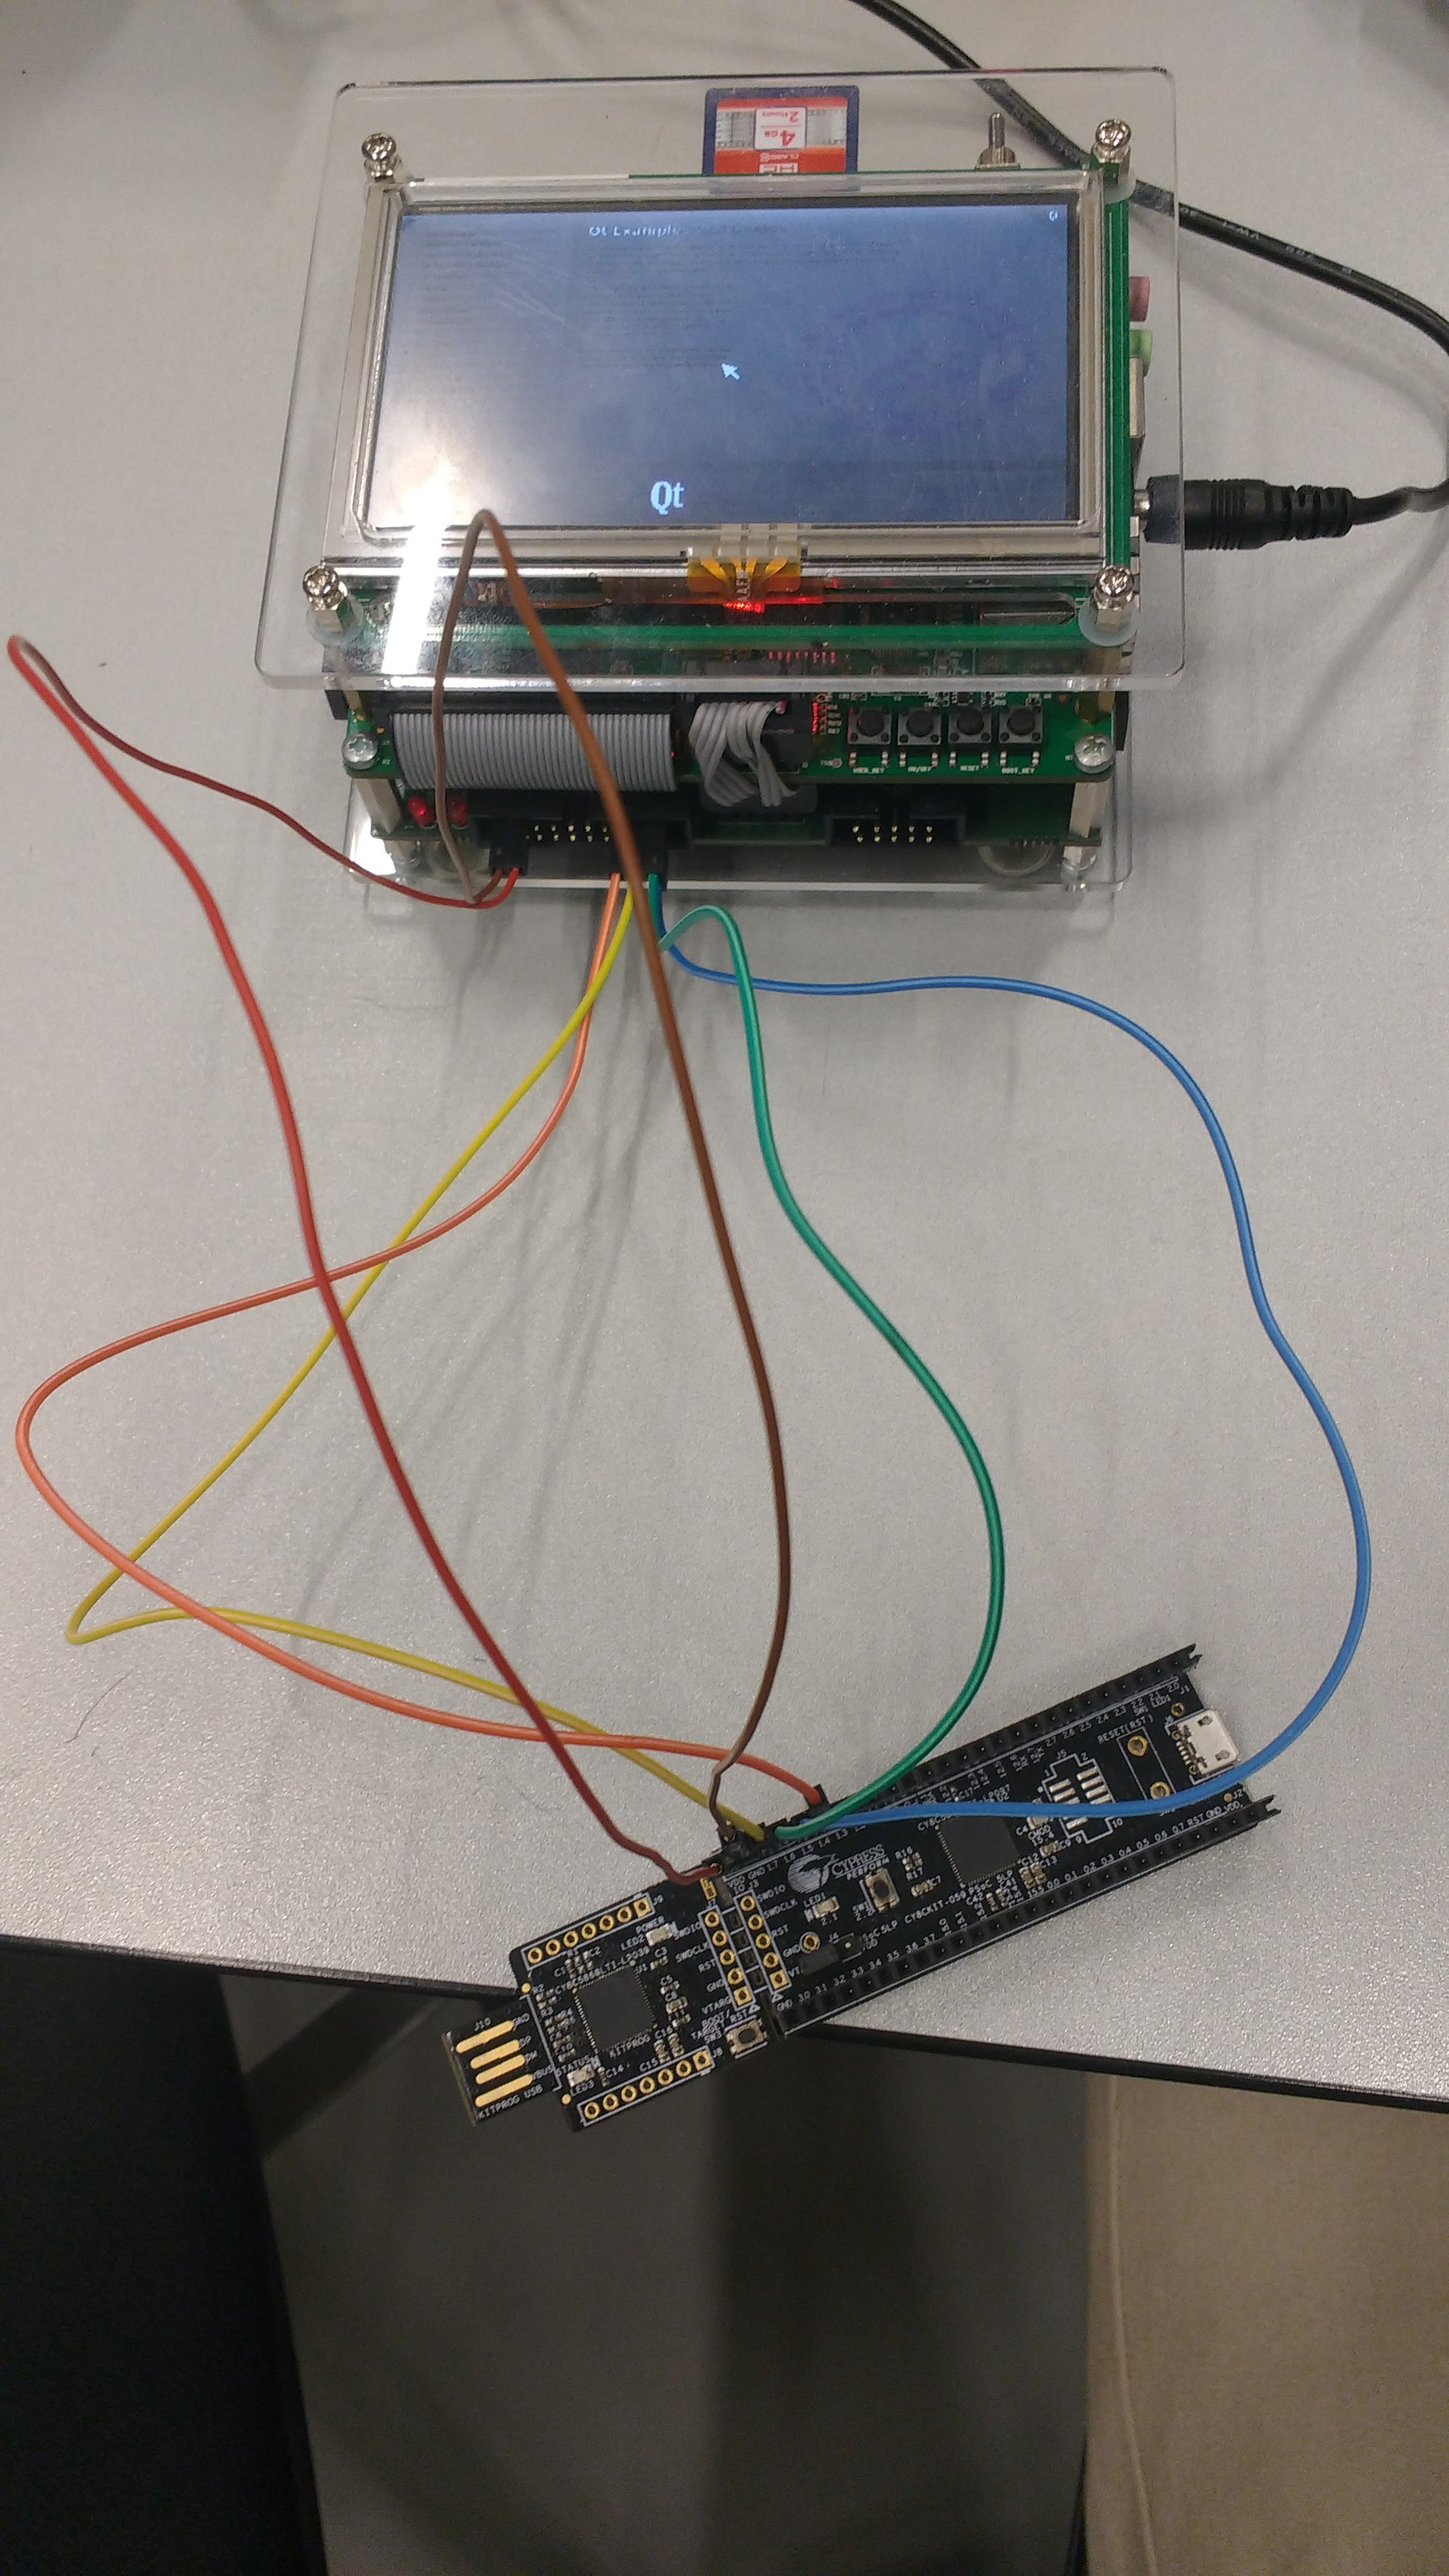
\includegraphics[scale=0.07]{tex/TeImRe/SPI/Realisering_devkit_psoc}}
	\caption{Den fysiske forbindelese mellem Devkit800 og PSoC Master}
	\label{ffm_DK8k_PSoC}
\end{figure}

Som nævnt i Design afsnittet for SPI\footnote{Se undersektion \ref{sub:SPI}}, har der ikke været adgang til koden for SPI device driveren på DevKit8000, hvorfor implementeringen
af denne ikke kan beskrives nærmere. \\

Til implementeringen af SPI på PSoC Master og PSoC Slave er der benyttet PSoC creator, som med et drag-and-drop interface gør det nemt at opsætte SPI forbindelsen. 
Derudover indeholder programmet en main fil hvori der er implementeret en håndtering af de modtagende databits. Koden består dybest set at en interrupt service 
rutine (ISR), som kaldes hver gang, der er blevet læst en data-byte ind på Rx-bufferen. Den tilhørende interrupt-rutine vil fungere som en state-machine, 
hvor den pågældende data-byte læses i en switch, som, alt efter kommandoen, sætter en variabel, der læses i PSoC'ens tilhørende \textit{main}-funktion, til en 
bestemt værdi. I \textit{main}-funktionen skal der da påkaldes de relevante metoder, som skal følge den modtagne kommando. Grunden til denne implementering er, 
at holde så meget af programmets funktionalitet så opdelt som muligt for at opretholde princippet om høj samhørighed - lav kobling. For mere information omkring 
koden for PSoC master og PSoC Slave henvises til bilag\footnote{Se kapitel 2 i Design, Implementering og Test}.